% !TeX root = ../../thesis.tex
\chapter{Conclusion}\label{ch:conclusion}


Each chapter of this thesis consists of an independent scientific study and includes its own detailed discussion. Consequently, this chapter provides a general summary and conclusion of the current PhD research. Moreover, it includes an overview of the limitation and challenges we needed to tackle during the project, as well as suggested future directions and contributions to continue this piece of work.

\section{Project summary}

% overview of chapters and objectives

This PhD thesis presented a mechanistic model of the biodegradation process of metallic biomaterials, with a focus on the \textit{in vitro} Mg biodegradation. For achieving this goal, the project was divided into several work packages, each of which containing a specific goal to reach, as described in Chapter \ref{ch:objective}. The research carried on in this PhD thesis lies where biomedical engineering, materials science, mathematics, and computational sciences collide. The relevant elements of these disciplines were employed in a multidisciplinary manner to deliver a multiphysics model of the chemistry of biodegradation by considering the effect of the environment determined by the final application. After developing the model, it has been used in multiple case-studies to demonstrate the integration capabilities, which was one of the initial goals of the project.

As stated in Chapter \ref{ch:introduction}, building a mechanistic model of the biomaterials biodegradation for any arbitrary shape in 3D can be challenging. Despite the technical challenges, such a model can provide more accurate predictions of the underlying processes in comparison to data-driven and stochastic models. In order to build the core computational model, the chemical reactions occurring at the interface of Mg during the biodegradation were converted to corresponding mathematical forms, a set of reaction-diffusion PDEs. Since studying the change of the morphology of the implants and medical devices can be beneficial for the design optimization processes, it was essential for the model to be able to capture the morphological changes in the shape of the simulated 3D objects. For doing this, an interface tracking technique, formulated using the level-set method, was integrated into the biodegradation model, enabling us to capture the movement of the corrosion front due to loss of materials. This model was capable of reproducing the basic biodegradation behavior of commercially-pure Mg in saline and buffered solutions, typical test environments to evaluate the corrosion behavior of metallic materials. 

Due to the complexity of the derived mathematical model, it was more convenient to implement it in an in-house code with full control on the details of numerical solution and computational implementation. More elaboration on this choice will be discussed in Section \ref{sec:open_source}. The resulting coupled equations were solved using the finite element method implemented in the open-source domain-specific language FreeFEM, in which a wide range of relevant scientific computing libraries were employed to performed sub-tasks such as mesh generation, mesh refinement, iterative solution of linear systems of equations, and preconditioning the models. The implementation and validation details are elaborated in Chapter \ref{ch:core}, where the evolved hydrogen gas during the corrosion process was used to calibrate the model, and global pH measured in immersion tests was used for validating it, for which a good agreement between the experimental and computational results was observed.

Extending the model to capture more complex forms of the biodegradation phenomenon could have been followed in various directions, like by adding the effect of alloying effects or modeling other types of localized corrosion such as pitting. However, instead of doing this, we decided to further develop the model for dealing with more complex chemistry of the surrounding environments such as electrolytes containing enormous chemical components. Doing this required having two extensions on the model: 1) adding the physics of fluid flow to make it possible to model more advanced experimental setups such as hydrodynamics and perfusion conditions, and 2) adding more contributing chemical components to the core computational model. For the former, efficient CFD codes for simulating the behavior of the circulating fluid flow were developed and coupled with the core biodegradation model, the details of which is discussed in Chapter \ref{ch:fluid}. For the latter extension, a thermodynamics-based code was coupled with the biodegradation model to predict the concentration of contributing chemical species according to the computed pH on the corrosion interface. Such coupling resulted to accurate predictions of local pH changes, which is elaborated was Chapter \ref{ch:kinetics}.

For increasing the accuracy of the employed level-set formalism, correlating the rate of material loss to the biodegradation velocity at which the interface shrinks, the generated mesh used for simulations was always adaptively refined on the corrosion front, resulting in computationally intensive models comprising of usually $\sim10-20\text{M}$ tetrahedral elements. Consequently, efficient HPC techniques, including partitioning the mesh and distributing the computational load among available computing resource, were employed in all the developed models. This reduced the simulation time in orders of magnitude. The details of this parallelization as well as the results of scaling tests to evaluate the behavior of the parallel model in HPC environments were presented in Chapters \ref{ch:hpc} and \ref{ch:cup}.

Moreover, the computational models and workflows developed as part of this PhD thesis were assembled together in a standalone software called BioDeg, which is available to download as an open-source tool for biodegradation simulation of any arbitrary 3D geometry. The software features a graphical user interface and a basic pre-processor, helping non-technical users to take advantage of its functionality in a user-friendly manner. Various aspects of the development of BioDeg are detailed in Chapter \ref{ch:biodeg}. Furthermore, the details and workflow developed for the calibration and parameter estimation of the developed biodegradation model was separately published as an open-source educational material. This was done using the Jupyter notebooks and open science principles, the details of which can be found in Chapter \ref{ch:bayesian}.

In the end, in order to demonstrate the capabilities of the developed biodegradation model in real-world applications and scenarios related to biomedical engineering, it was used in a couple of case-studies. In these case-studies, the biodegradation model was coupled or integrated with other models to simulate more comprehensive phenomena. The case-studies selected to present in this PhD thesis include investigating the mechanical loosening of jaw bone plates (Chapter \ref{ch:mandible}), biodegradation of personalized printed porous implants (Chapter \ref{ch:cup}), and mechanical integrity of infilled structures during the biodegradation process (Chapter \ref{ch:infill}).



\section{General discussion, challenges, and limitations}

\subsection{Role of open-source tools and open science} \label{sec:open_source}

% open source, the benefits, tuxriders, education
% figure of empoyed tools

Open-source paradigm and open science principles, played an important role in the carried out research in this PhD. Without the added value of open-source tools, it was literally impossible to build a multiphysics moving boundary model which was later used to perform a simulation with over 45M elements on 7000 CPU cores (as presented in Chapter \ref{ch:cup}). The added values of open-source comprise the potential flexibility required by computational science project, open standards and exchange formats required for integration and interoperability of models, availability of tools for almost every aspect of model development, responsive support provided by open-source communities, and increasing transparency. These advantages will be elaborated in this section.

Implementing the mathematical model derived from the chemistry of biodegradation, which was also coupled with other physical problems such as the perfusion effect, needed flexibility and full control on numerical details. As a result, doing such implementation in commercial tools with pre-built models such as ANSYS, Abaqus, and COMSOL would have been very inefficient and prone to wasting resources and time. Even though certain customization features such as user subroutines in Abaqus and weak form interface in COMSOL are available to provide some flexibility in model implementation, the possible modification level does not meet our requirements and would decrease work productivity and efficiency of models. Instead, we decided to opt a different approach, bringing freedom in development of the intended large-scale mechanistic model of the biodegradation behavior for any arbitrary 3D shape. For doing this, a broad range of relevant open-source tools and libraries were leveraged in various aspects of this PhD to obtain desired numerical accuracy in high-performance computational models, such as mesh generation and refinement, geometry construction, preconditioning, weak form implementation, solution of derived linear systems, parameter estimation, and postprocessing. An overview of these tools is presented in Fig. \ref{fig:conclusion_tools}.

\begin{figure}[h]
\centering
\medskip
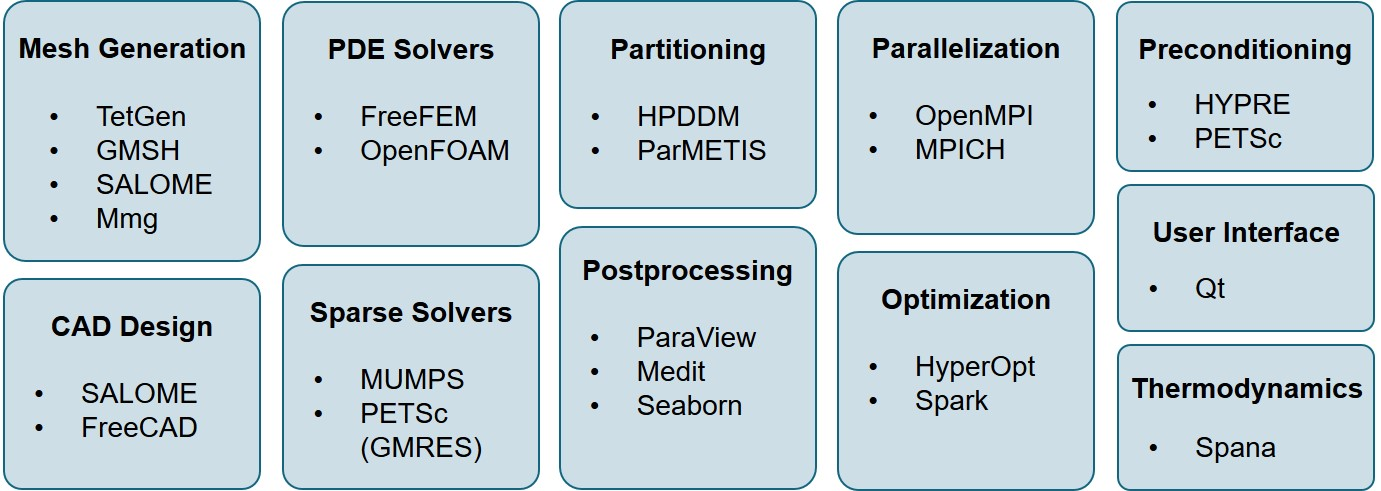
\includegraphics[width=\textwidth]{tools.jpg}
\caption[Overview of open-source tools and libraries used in this PhD]{An overview of tools and libraries used in this research, which are all free and open-source.} \label{fig:conclusion_tools}
\end{figure}

One of the biggest advantages of most of the open-source tools in the scientific computing community is related to the openness of standards and exchange formats. Combined with the flexibility allowed by these tools for doing any desired customization, this characteristic makes almost any coupling or exchange possible among various tools. This means that no matter if it is officially supported by the developers or not, the output of any tool can be used as the input of anther one. This flexibility was a big advantage for the research done in this PhD in different levels. There are many examples to mention here from all the chapters. The mesh generation done in Chapter \ref{ch:cup} is a good large-scale example, which was done using a combination of FreeFEM internal mesh engine, Mmg, GMSH, and MeshLab on the output of a CGAL-based code. Another relevant example can be the geometry processing and mesh preparation done done in Chapters \ref{ch:core}, \ref{ch:fluid}, and \ref{ch:kinetics}, where an orchestration of various tools, like SALOME, GMSH, meshio, and FreeFEM made it possible to generate a high-detailed large-scale multi-material mesh for the biodegradation and fluid flow simulations. 

The flexibility level provided by open-source tools is not comparable to commercial software programs. This brings two main benefits into play: 
\begin{enumerate}
\item
Easier customization to adapt to the target application and usage, which can be observed in various levels. The most-known flexibility in this regard is related to the availability of source codes, making it possible for any researcher to modify the tool to work in a desired manner. Such modifications were useful in some stages of the current PhD, where slight changes were made to some of the interfaces of FreeFEM to behave differently. However, this level is not the only flexibility useful for computational projects. Another prominent possibility is the customization during the build process of the software, meaning that various features of the employed tools can be customized while compiling them from source codes. This is beneficial from the performance perspective too, where building the software from the source codes optimizes it depending the software and hardware configuration of the target system, which contributes to increasing the performance and efficiency of the tool. This will be discussed in more details in Section \ref{sec:conclusion_hpc}.
\item
More responsive community formed around the tool, providing different levels of help and support for solving users' issues and developing new features. These communities are unique for open-source paradigm as the contributors are not necessarily the main software developers. This fact relies on the openness nature of the software, making it possible for anyone to contribute to the different forms of support. This is extremely important and beneficial for more complex tools like the ones typically used in the scientific computing and computational science projects. 
\end{enumerate}

Another added value of using open-source tools is related to the transparency and reproduciblity of the research, a bonus that opens the stage for more efficient science outreach as well. When a research is constructed using tools that are freely available, it means that re-run the codes and models to reproduce the results, an action that dramatically increase the transparency of the research and trust in the obtained results. This is still possible in research studies done with proprietary software programs, but the users trying to reproduce the results should have paid for the licenses first. Moreover, the tendency to share the codes, models, and workflows is more in the open-source community, which is another reason why this reproduciblity concerns is less popular among the proprietary software users. As mentioned above, this added value has a mutual-benefit for booth the transparency and science outreach, meaning that sharing the developed models and worklfows can be treated as efficient project outreach in addition to increasing the trust and transparency. In other words, open-source tools can help  project outreach activities meet open science principles. An example of these activities are presented in Chapters \ref{ch:biodeg} and \ref{ch:bayesian}. In Chapter \ref{ch:biodeg}, the developed models are encapsulated into a standalone open-source software which relies on open-source tools to work, implying that the users do not need any additional license to run biodegradation simulations. This software was reviewed by and published in the Journal of Open-Source Software (JOSS) \cite{Barzegari2022JOSS}. In Chapter \ref{ch:bayesian}, the details of the utilized parameter estimation process, an important building block of the carried out research, was represented as a self-teaching educational material in the format of Jupyter notebooks. This work was published in the Journal of Open-Source Education (JOSE) \cite{Barzegari2021JOSE}. 

As a summary, we should emphasize that this PhD was not possible without the freedom and flexibility available in open-source scientific computing world. The open-source paradigm also helped us to increase the outreach of the project using open science principles. Additionally, it's worth mentioning that in line with the project outreach activities, the obtained knowledge is getting published as a YouTube project called TuxRiders\footnote{\url{https://www.youtube.com/TuxRiders}}, in which the power of open-source scientific computing tools are discussed in details and demonstrated using practical use cases coming from real-world projects, which encompasses the research carried out in this PhD as well.



\subsection{Moving interface problems}

% defining BCs on an implicit interface
Although the interface tracking method used in the developed biodegradation model had prominent advantages, from the implementation perspective, it was one of the biggest challenges in all aspects of the modeling work carried out in this research. The challenge became boosted by considering the necessity of parallel computing and partitioned meshes. Moreover, integrating interface-coupled problems such as mass transfer and fluid flow can be quite challenging in presence of an interface tracking scheme. 

In this PhD, a level-set formalism was employed to track the moving corrosion front, making it possible to investigate the morphological changes of the desired 3D degrading object. This was for sure one of the unique aspects of the current model in comparison to other degradation and corrosion models which usually deal with simplified representation of geometries in 2D. However, some implementation hurdles were inevitable to achieve this uniqueness, which can be discussed from the computational resource consumption perspective as well. Some of the arising challenges are already elaborated in Section \ref{sec:hpc_ls_issues}.

In the developed level-set formalism, an implicit distance function was used such that its zero iso-surface represents the interface. This implicit function was calculated as a solution of the level-set PDE, in which the interface shrinkage velocity was correlated to the gradient of the released ions concentration. This PDE was solved in each time step along with the other PDEs derived from the chemistry of biodegradation and other coupled physics. The main challenge emerges due to the way that the boundary conditions of the coupled problems are defined. The boundary conditions are related to the mass transfer problem and should be defined on the biodegradation interface, which is moving with as the level-set implicit function evolves. All in all, this means that the BCs of the system are defined on the solution of one of the governing equations, which makes the implementation and debugging complex, especially in 3D. 

Two other factors can make this challenge even more complex: 1) the necessity of HPC and partitioning the mesh, and 2) adding more physics to the core problem such as presence of fluid flow affecting the mass transfer problem, based on which the level-set formalism is constructed. The current research faced these challenges in all the chapters of this thesis, which required spending time on debugging the behavior of the developed interface tracking model. This required even more time when an addition to the underlying physics was under development, such as the works presented in Chapters \ref{ch:fluid}, \ref{ch:kinetics}, and \ref{ch:infill}.

The employed HPC and mesh partitioning techniques, including the mesh decomposition preconditioners in HPDDM library and parallel computing features of PETSc toolkit elaborated in Chapter \ref{ch:hpc}, are capable of handling the solution of the level-set equation in parallel without any major problem. However, a well-known problem of the level-set method causes a big issue here. Since advecting the implicit distance function causes perturbation in its numerical solution, the function should be re-initialized after a couple of time steps. But, doing this re-initialization on a partitioned mesh is almost impossible, making it necessary to gather the distributed partitions again back into a global mesh before doing the re-initialization. Doing this decreases the overall parallel efficiency of the model in large-scale model, more details of which can be found  in Section \ref{sec:hpc_ls_issues}.

Another relevant challenge worth mentioning here was related to coupling multiple interface tracking methods. An example of this is presented in Chapter \ref{ch:tissue}, where the final goal was to couple the level-set-based model of biodegradation with a developed phase-field model of tissue growth. As mentioned above, defining BCs on the solution of one of the governing equations (the level-set PDE in this case) can be quite challenging. For coupling multiple moving interface models, one model should be declared on the solution of another one, which is a more complicated problem in comparison to the problem described for the BCs. More details of this problem are elaborated in Section \ref{sec:tissue_challenges}. Another example presented in this thesis can be found in Chapter \ref{ch:infill}, in which the biodegradation model was coupled with the level-set-based mechanical integrity model, meaning that two level-set functions were defined to describe different phenomena.

\subsection{High-performance computing and scaling} \label{sec:conclusion_hpc}

%Building with different MPI implementations
%Inter-node communication
%Running parallel FF
%Mesh generation (parallel, sequential)
%Converting surface mesh to volume
%Scaling issues
%Memory issues
%Node types
%Visualization, GPU nodes
%Partitioning (METIS, ParMETIS)
%Storage
%Solving NS equation

\subsection{Representing the chemistry in mechanistic models}

% capturing the chemistry in math
% lack of certainty in chemical experiments, leading to difficulty in modeling

The core of this PhD research was related to capturing the chemistry of biodegradation process in mathematical forms as realistic as possible. There is a wide variety of different approaches for doing so \cite{Abdalla2020}. The available methods can be classified in different ways, but one of the most representative classifications is to divide them into mechanistic and phenomenological approaches. In mechanistic models, also called physical models, it is the physical rules that are captured by the model. In contrast, in phenomenological modeling, the underlying physics is represented by simplified empirical relationship of phenomena to each other. 

The developed model in this PhD falls in the category of mechanistic models, describing the underlying chemistry by a set of PDEs. Although these model provide more insightful information about the occurring phenomena and are easier to validate compared to phenomenological models, they bring another challenge into play: the phenomena should be well known and investigated so that it can be converted by the mathematical forms. Mapped to the chemistry that the current model tries to capture, this challenge can be divided into two independent issues: 1) obtaining numerical values for all chemical parameters, some of which are difficult to get in experiments, and 2) lack of certainty in chemical experiments. These challenges are elaborated below.

Converting the chemical reactions of the biodegradation process to a mechanistic computational model results in a model with multiple parameters. In a reaction-diffusion system, such as the one developed in this PhD, these parameters are related to the diffusion coefficient of the transport of contributing components and the reactions rates at which the chemical reactions are happening. Measuring the exact value of these parameters is almost impossible in experimental studies, especially for complex systems like the Mg degradation in SBF solutions, where there are a lot of interactions between the different components of the system. This measurement is more complicated for the reaction rates since it is difficult to isolate a single reaction among all the correlated reactions occurring in a complex phenomenon like the biodegradation process and measure its rate. The common solution to this problem is the so called parameter estimation or model calibration process, in which the model parameters are optimized using an appropriate routine to reproduce the experimentally-obtained output. Depending on the number of parameters and the chemistry that the mechanistic model is representing, this process can become complex soon, loosing part of its efficiency to yield to correct values for the physical and chemical coefficients. This issue is detailed in Chapter \ref{ch:core}. Moreover, an overview of the necessity of the parameter estimation process can be found in Chapter \ref{ch:bayesian}.

The uncertainty in chemical reactions might not be an issue in phenomenological models, but it is a big challenge in mechanistic modeling. An example of lack of certainty in chemistry of the biodegradation process is the unknown composition of the precipitation layer forming in complex electrolytes such as SBF and HBSS. The absence of a known composition makes it impossible to construct a mechanistic computational model of the precipitation process because it needs the stoichiometry of the reactions as the coefficients of the derived reaction-diffusion differential equations. This problem is elaborated in Chapter \ref{ch:kinetics}, where a solution is proposed for tacking it in which a thermodynamics-based code is coupled with the mechanistic biodegradation model to provide more information of the concentration of involved chemical components on the biodegradation surface. Another example for this issue can be the high variability of the experimental results to the composition of the tested materials. As presented in Chapter \ref{ch:kinetics}, even with a slight change in the alloying composition, like by going from highly-pure Mg to commercially-pure Mg, the results obtained for local pH profiles change significantly. These observations, which do not have a solid theoretical description from the chemical perspective, are extremely difficult to capture and mimic in mechanistic models such that the computational predictions reproduce the experimentally-obtained results. 




\section{Future perspectives}



%%%%%%%%%%%%%%%%%%%%%%%%%%%%%%%%%%%%%%%%%%%%%%%%%%
% Keep the following \cleardoublepage at the end of this file, 
% otherwise \includeonly includes empty pages.
\cleardoublepage

% vim: tw=70 nocindent expandtab foldmethod=marker foldmarker={{{}{,}{}}}
